\section{Self Attention Layer}
\begin{frame}{}
    \LARGE Advanced Computer Vision: \textbf{Self Attention Layer}
\end{frame}

\begin{frame}{Self-Attention Mechanism}
    \begin{itemize}
        \item \textbf{Self-Attention:} Computes attention within a single sequence.
        \item \textbf{How it works:}
        \begin{itemize}
            \item Each token attends to every other token.
            \item Captures global context, not just local dependencies.
        \end{itemize}
    \end{itemize}
\end{frame}

\begin{frame}{Self Attention Layer}
\begin{columns}
    
    \begin{column}{0.6\textwidth}
    \only<1>{
    \begin{figure}
    \centering
    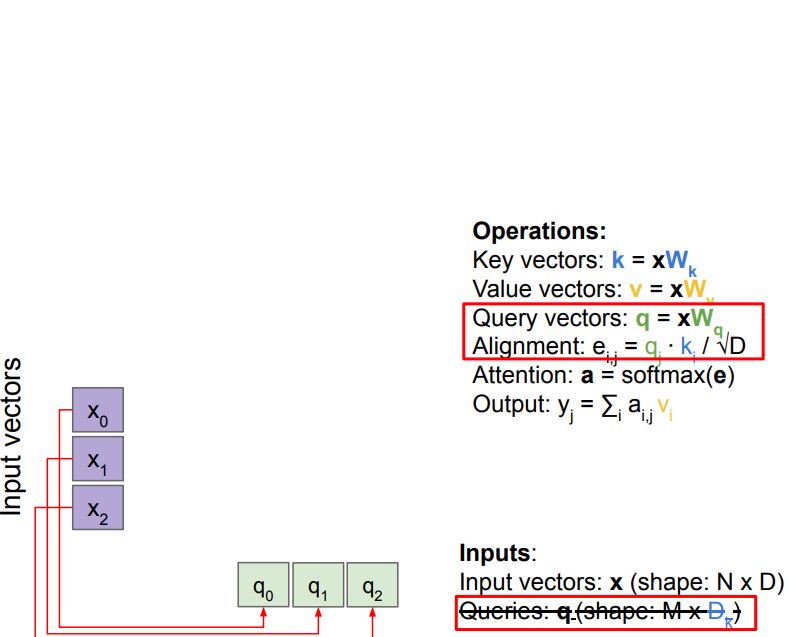
\includegraphics[width=1.0\textwidth,height=1.0\textheight,keepaspectratio]{images/advanced-cv/attention_27.png}
    \end{figure}
    }

    \only<2>{
    \begin{figure}
    \centering
    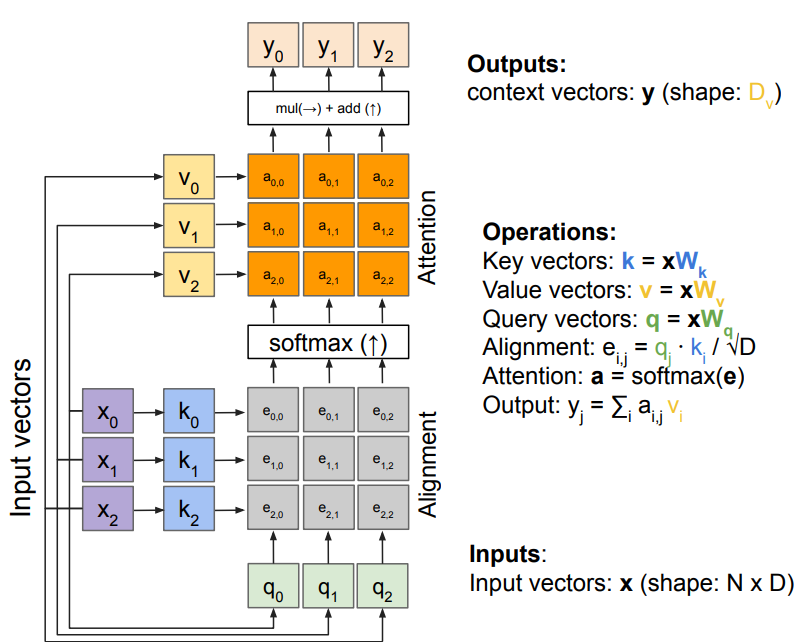
\includegraphics[width=1.0\textwidth,height=1.0\textheight,keepaspectratio]{images/advanced-cv/attention_28.png}
    \end{figure}
    }

    \only<3>{
    \begin{figure}
    \centering
    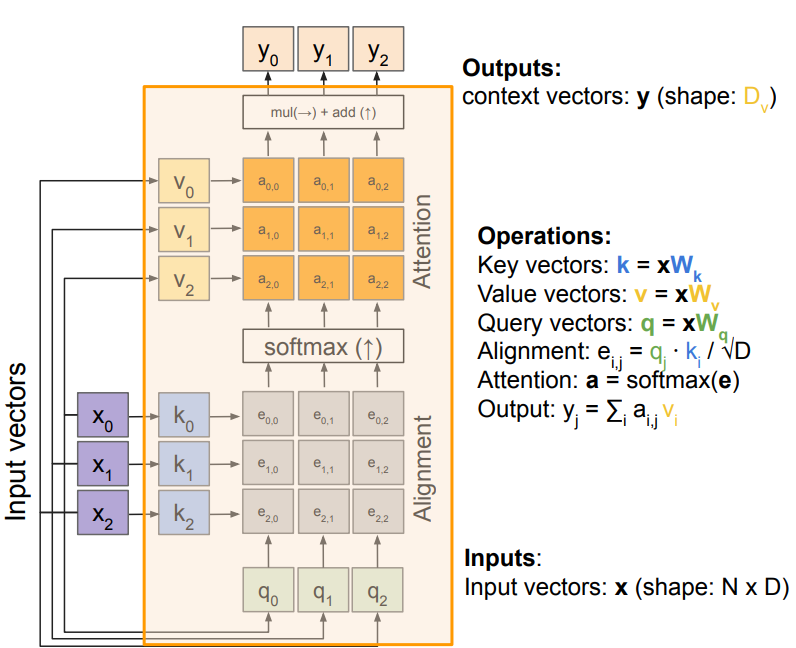
\includegraphics[width=1.0\textwidth,height=1.0\textheight,keepaspectratio]{images/advanced-cv/attention_29.png}
    \end{figure}
    }
        
    \end{column}

    \begin{column}{0.5\textwidth}
    \only<1-2>{
    \begin{itemize}
        \item Recall that the query vector is a function of the input vectors.
        \item We can calculate the query vectors from the input vectors, thus defining a "self-attention" layer.
        \item There are no input query vectors anymore.
        \item Instead, query vectors are calculated using a fully connected (FC) layer.
    \end{itemize}
    }


    \only<3>{
    \begin{figure}
    \centering
    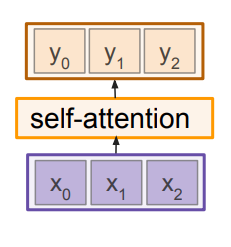
\includegraphics[width=0.5\textwidth,height=1.0\textheight,keepaspectratio]{images/advanced-cv/attention_30.png}
    \end{figure}
    }
    
    \end{column}
\end{columns}
\end{frame}